\documentclass[11pt]{standalone}
\usepackage{tikz}
\usetikzlibrary{angles, calc, decorations.pathmorphing, quotes, spy}

\begin{document}
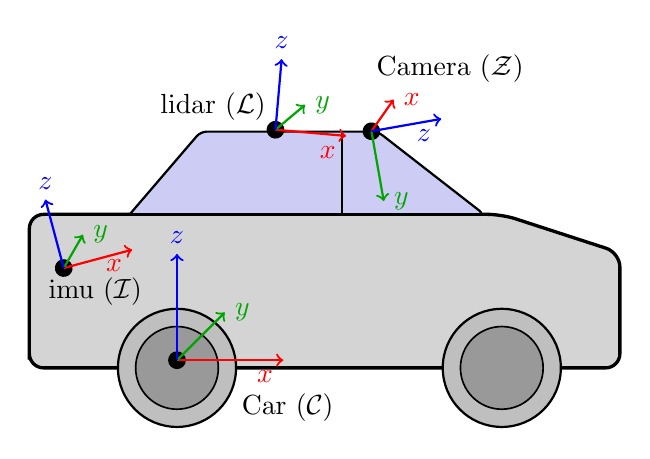
\begin{tikzpicture}[scale=1.5]
    % Define car parameters
    % Car height
    \def\ch{2}
    % Car length
    \def\cl{5}
    % Car body height
    \def\bh{\ch*0.65}
    % Roof length
    \def\rl{\cl*0.6}
    % Roof height
    \def\rh{\ch*0.35}
    % Car tilt angle
    \def\ct{6}
    % Anchor point is southwest
    \coordinate (b) at (0,0);
    % Offset to roof and wheels
    \coordinate (r) at ($(b) +(\cl*0.17,\ch*0.65)$);
    \coordinate (w) at ($(b) + (\cl*0.25,0)$);

    % Body
    \draw[black, fill=black!17, rounded corners=1.2ex, very thick]
    (b) -- ++(0,\bh) -- ++(\cl*1/5,0) --  ++(\cl*3/5,0) -- ++(\cl*1/5,-\bh*0.25)
    -- ++(0, -\bh*0.75) -- (b) -- cycle;
    % Roof
    \draw[very thick, rounded corners=0.5ex, fill=black!20!blue!20!white,thick]
    (r) -- ++(0.2*\rl,\rh) -- ++(0.5*\rl,0) -- ++(0.3*\rl,-\rh) -- (r);
    % \draw[thick] ($(r) + (\cl*0.5,\bh)$) -- ++(0,\rh);
    \draw[thick] (r)++(\rl*0.6,0) -- ++(0,\rh);

    % Wheels
    \draw[draw=black,fill=gray!50,thick] (w) circle (.5);
    \draw[draw=black,fill=gray!50,thick] (w) ++(\cl*0.55,0) circle (.5);
    % Inner wheels
    \draw[draw=black,fill=gray!80,semithick] (w) circle (.35);
    \draw[draw=black,fill=gray!80,semithick] (w) ++(\cl*0.55,0) circle (.35);

    % Car middle point
    \coordinate (m) at (\cl*0.25, \bh*0.05);
    \filldraw (m) circle (2pt) node[below right, xshift=0.7cm, yshift=-0.3cm] {Car ($\mathcal{C}$)};
    % Coordinate frames
    \draw[thick,->, red] (m) -- ++(0.9,0,0) node[anchor=north east]{$x$};
    \draw[thick,->, black!35!green] (m) -- ++(0,0,-1.05) node[anchor=west]{$y$};
    \draw[thick,->, blue] (m) -- ++(0,0.9,0) node[anchor=south]{$z$};

    % IMU middle point (random)
    \begin{scope}[rotate=15]
        \coordinate (mi) at (\cl*0.1, \bh*0.57);
        \filldraw (mi) circle (2pt) node[below, xshift=0.4cm] {\glsentryshort{imu} ($\mathcal{I}$)};
        % Coordinate frames
        \draw[thick,->, red] (mi) -- ++(0.6,0,0) node[anchor=north east]{$x$};
        \draw[thick,->, black!35!green] (mi) -- ++(0,0,-0.6) node[anchor=west]{$y$};
        \draw[thick,->, blue] (mi) -- ++(0,0.6,0) node[anchor=south]{$z$};
    \end{scope}

    % LIDAR middle point (random)
    \begin{scope}[rotate=-5]
        \coordinate (ml) at (1.9, 2.19);
        \filldraw (ml) circle (2pt) node[above left] {\glsentryshort{lidar} ($\mathcal{L}$)};
        % Coordinate frames
        \draw[thick,->, red] (ml) -- ++(0.6,0,0) node[anchor=north east]{$x$};
        \draw[thick,->, black!35!green] (ml) -- ++(0,0,-0.6) node[anchor=west]{$y$};
        \draw[thick,->, blue] (ml) -- ++(0,0.6,0) node[anchor=south]{$z$};
    \end{scope}

    % Camera middle point (random)
    \begin{scope}[rotate=10]
        \coordinate (ml) at (3.2, 1.47);
        \filldraw (ml) circle (2pt) node[above, xshift=1cm, yshift=0.5cm] {Camera ($\mathcal{Z}$)};
        % Coordinate frames
        \draw[thick,->, red] (ml) -- ++(0,0,-0.6) node[anchor=west]{$x$};
        \draw[thick,->, black!35!green] (ml) -- ++(0,-0.6,0) node[anchor=west]{$y$};
        \draw[thick,->, blue] (ml) -- ++(0.6,0,0) node[anchor=north east]{$z$};
    \end{scope}
\end{tikzpicture}
\end{document}